%%%%%%
%
% $Autor: Wings $
% $Datum: 2020-01-18 11:15:45Z $
% $Pfad: githubtemplate/Template/Presentations/Template/slides/rename.tex $
% $Version: 4620 $
%
%
% !TeX encoding = utf8
% !TeX root = Rename
%
%%%%%%


\Mysection{System Visuals}
\STANDARD{JetBot System}
{
\begin{figure}
	\centering
	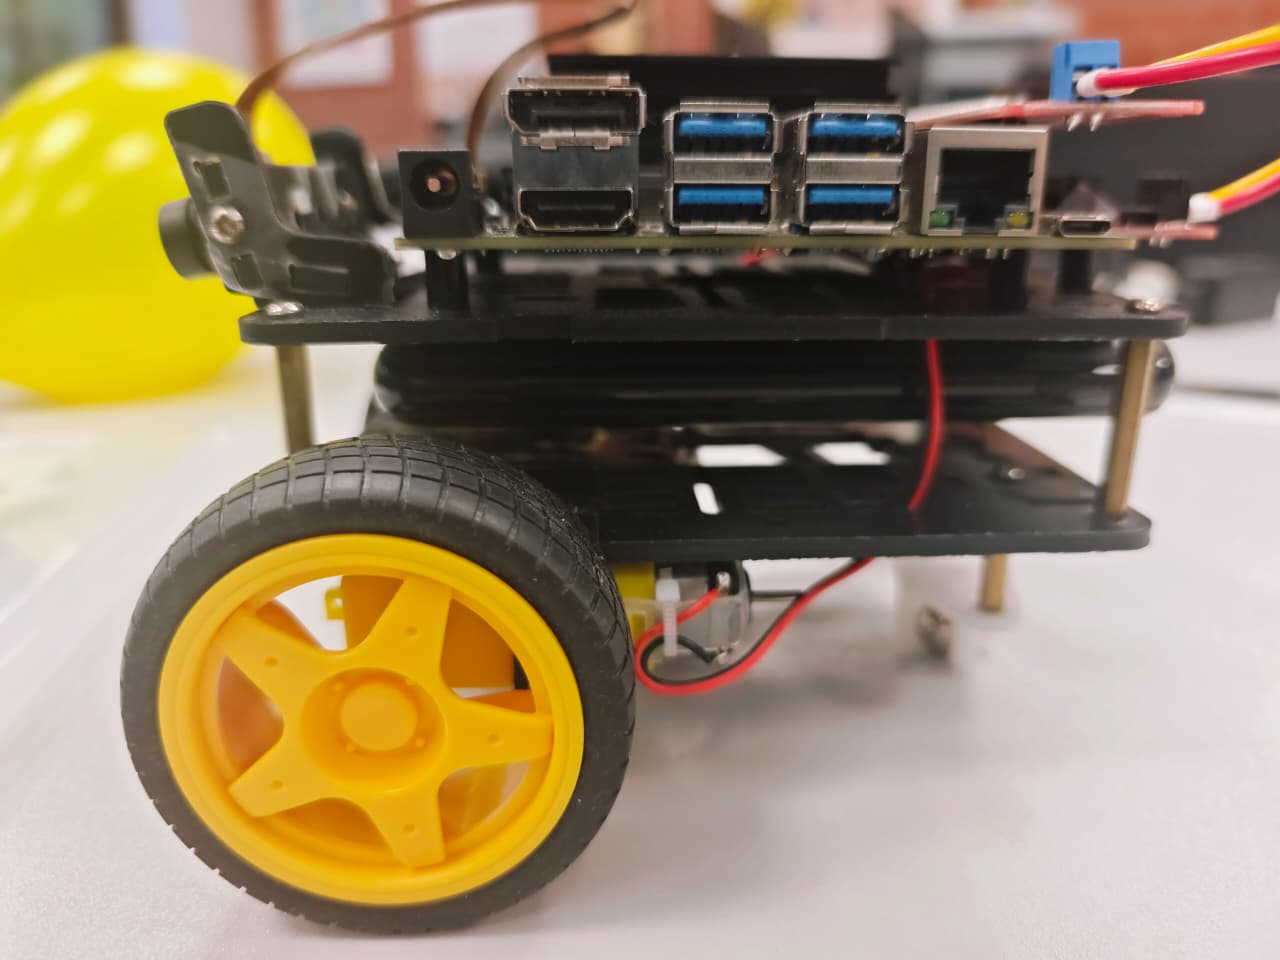
\includegraphics[width=0.7\linewidth]{images/MBSideView}
	\caption{Sytem Side View}
	\label{fig:mbsideview}
\end{figure}
}
\STANDARD{JetBot System Top View}{
\begin{figure}
	\centering
	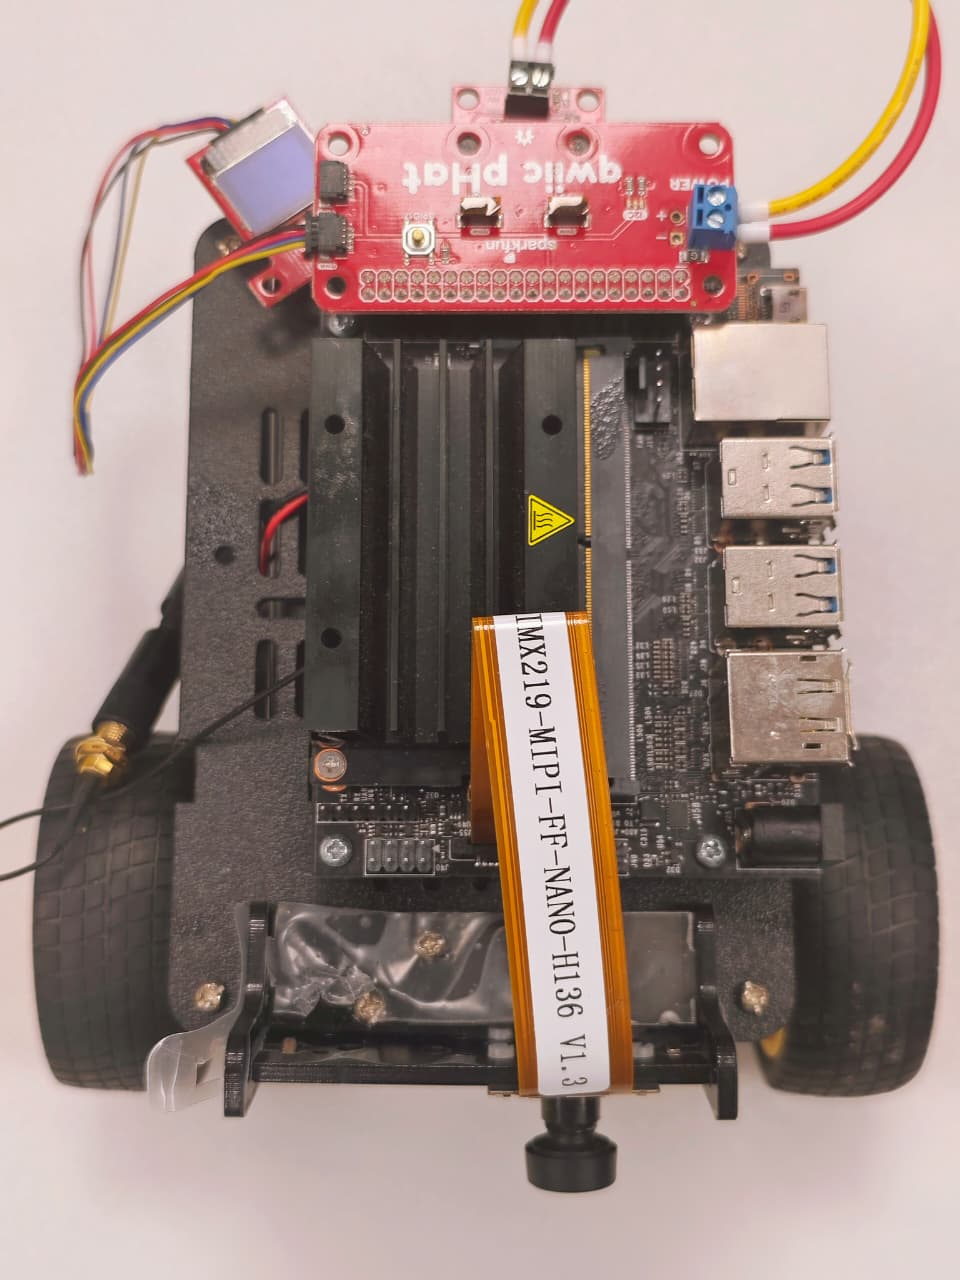
\includegraphics[width=0.4\linewidth]{images/MBTopView}
	\caption{System Top View}
	\label{fig:mbtopview}
\end{figure}
}

\STANDARD{JetBot System Front View}{
\begin{figure}
	\centering
	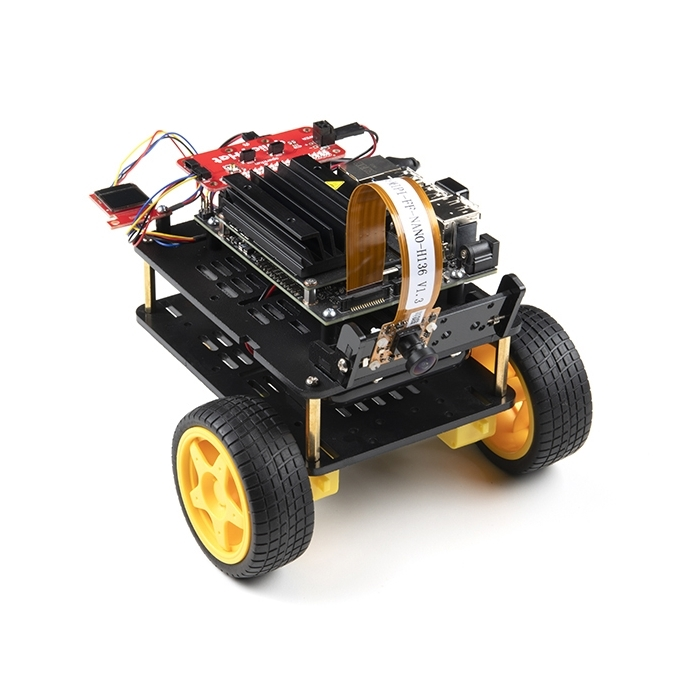
\includegraphics[width=0.5\linewidth]{images/SparkFunJetBotAIKitFront}
	\caption{System Front View}
	\label{fig:sparkfunjetbotaikitfront}
\end{figure}
}
\STANDARD{JetBot System Back View}{
	\begin{figure}
		\centering
		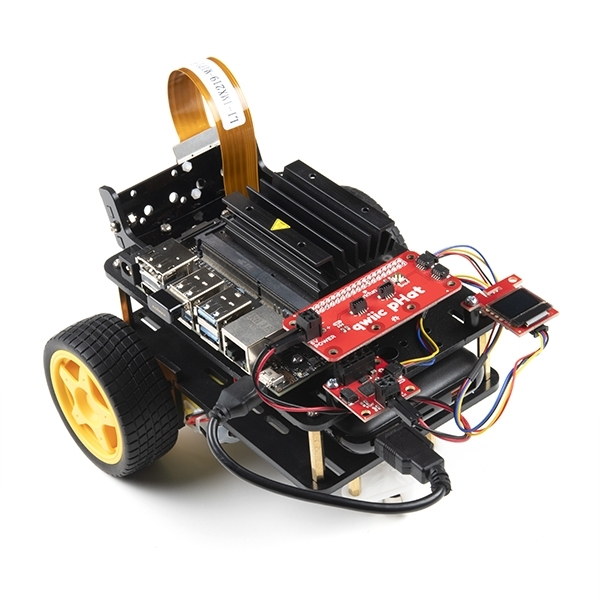
\includegraphics[width=0.5\linewidth]{images/SparkFunJetBotAIKitBack}
		\caption{System Back View}
		\label{fig:sparkfunjetbotaikitback}
	\end{figure}
}
\Mysection{First Steps}
\STANDARD{Connections}{
	\begin{enumerate}
		\item Insert the pre-flashed 64GB microSD card into the Jetson Nano.
		\item Connect the Leopard Imaging IMX219 CSI ribbon to CAM0; ensure contacts face inward.
		\item Mount and connect the Qwiic Motor Driver to the Qwiic bus; attach motors.
		\item Connect Edimax USB WiFi, keyboard, mouse, and HDMI/DP display.
		\item Connect recommended 5V @ 4A regulated power supply and power on.
		\item Confirm OS boots and JetBot localization image loads.
	\end{enumerate}
}
\STANDARD{First Steps}{
	\begin{enumerate}
		\item Power on the JetBot system using a stable 5V–4A power supply.
		\item Wait for Ubuntu to fully boot into the desktop environment.
		\item Log in with your configured username and password.
		Username:msr Password:msr
		\item Verify WiFi connection (top-right network icon or \texttt{nmcli device status}).
		\item Open a terminal and confirm camera detection:
		\begin{itemize}
			\item \texttt{dmesg | grep -i camera}
			\item \texttt{ls /dev/video*}
		\end{itemize}
		\item Launch Jupyter Notebook:
		\begin{itemize}
			\item Navigate to JetBot directory
			\item Run \texttt{jupyter notebook}
		\end{itemize}
	\end{enumerate}
}
\STANDARD{First Steps - Inside System}{
		\begin{enumerate}
		\item Open the Ground Localization notebook or application script.
		\item Run camera preview cell to confirm live feed.
		\item Execute calibration routine if first-time setup.
		\item Start localization demo or main control script.
		\item Verify:
		\begin{itemize}
			\item Live camera feed is active
			\item Localization status shows “OK”
			\item Motors respond to control commands
		\end{itemize}
		\item Use UI controls to Start / Stop / Calibrate as needed.
	\end{enumerate}
}

%%%%%%%%%%%%%%%%%%%%%%%%%%%%%%%%%%%%%%%%%%%%%%%%%%%%%%%%%%%%%%
\STANDARD{Setup}{
	\begin{itemize}
		\item Complete Ubuntu initial setup (locale, user, updates).
		\item Open a terminal and verify camera is detected (e.g. \texttt{dmesg | grep -i camera}).
		\item Run quick camera test (OpenCV or GStreamer preview).
		\item Start the JetBot localization demo / Jupyter notebook.
		\item Perform a short calibration run over representative ground textures.
	\end{itemize}
}


\Mysection{Main Function}
%%%%%%%%%%%%%%%%%%%%%%%%%%%%%%%%%%%%%%%%%%%%%%%%%%%%%%%%%%%%%%
\STANDARD{Main Function}{
	\begin{itemize}
		\item Capture continuous ground-facing images via IMX219 camera.
		\item Extract the visual features from ground texture (keypoints / descriptors).
		\item Compute frame-to-frame motion using visual odometry (VO).
		\item Fuse VO into a pose estimator and provide incremental localization updates.
		\item Output pose and velocity to motion controller for closed-loop navigation.
	\end{itemize}
}

%%%%%%%%%%%%%%%%%%%%%%%%%%%%%%%%%%%%%%%%%%%%%%%%%%%%%%%%%%%%%%

%%%%%%%%%%%%%%%%%%%%%%%%%%%%%%%%%%%%%%%%%%%%%%%%%%%%%%%%%%%%%%
\STANDARD{Help}{
	\begin{itemize}
		\item Use the built-in \textbf{Help} menu in the UI for quick-start steps and diagnostics.
		\item Online resources: JetBot GitHub, NVIDIA Jetson forums, SparkFun documentation.
		\item Local troubleshooting logs: \texttt{/var/log/syslog}, \texttt{dmesg}, and ROS topic logs.
		\item Contact support: provide system image version, microSD serial, and captured logs.
	\end{itemize}
}

%%%%%%%%%%%%%%%%%%%%%%%%%%%%%%%%%%%%%%%%%%%%%%%%%%%%%%%%%%%%%%
\STANDARD{Functions}{
	\begin{itemize}
		\item \textbf{Localize}: continuous pose estimation relative to ground features.
		\item \textbf{Calibrate}: camera intrinsic calibration and ground-texture sampling routine.
		\item \textbf{Record}: save camera frames and computed poses for offline analysis.
		\item \textbf{Play}: replay recorded sessions in the UI for debugging.
		\item \textbf{Export}: export calibration parameters and logs (JSON / NPZ).
	\end{itemize}
}

%%%%%%%%%%%%%%%%%%%%%%%%%%%%%%%%%%%%%%%%%%%%%%%%%%%%%%%%%%%%%%
\STANDARD{Maintenance}{
	\begin{itemize}
		\item Monthly: inspect and reseat CSI ribbon and Qwiic connectors.
		\item Every 3 months: re-run calibration if the robot undergoes mechanical changes.
		\item Keep software updated: apply tested JetPack / JetBot image updates only.
		\item Replace power adapter if voltage drops or frequent resets occur.
		\item Clean camera lens with microfiber cloth; avoid solvents.
	\end{itemize}
}

%%%%%%%%%%%%%%%%%%%%%%%%%%%%%%%%%%%%%%%%%%%%%%%%%%%%%%%%%%%%%%
\STANDARD{Troubleshooting}{
	\begin{itemize}
		\item \textbf{No camera preview}: reseat FFC ribbon (contacts inward), reboot, check \texttt{dmesg}.
		\item \textbf{Low FPS / lag}: verify power supply, reduce resolution, check CPU/GPU utilization.
		\item \textbf{Localization drift}: collect diverse calibration samples, improve lighting, enable feature filtering.
		\item \textbf{Motors jitter}: inspect motor wiring, verify motor driver current limits, update PID gains.
		\item \textbf{Network unreachable}: reconfigure WiFi or use wired Ethernet adapter.
	\end{itemize}
}

%%%%%%%%%%%%%%%%%%%%%%%%%%%%%%%%%%%%%%%%%%%%%%%%%%%%%%%%%%%%%%
\STANDARD{Specifications}{
	\begin{itemize}
		\item \textbf{Compute}: NVIDIA Jetson Nano Developer Kit (Quad-core ARM A57, 128-core Maxwell GPU).
		\item \textbf{Camera}: Leopard Imaging IMX219, 3280×2464 px, 136° FOV, MIPI CSI-2 (2-lane), up to 21 FPS at full res.
		\item \textbf{Storage}: 64GB microSD pre-flashed image.
		\item \textbf{Power}: 5V recommended, 4A for full AI workloads.
		\item \textbf{Connectivity}: AC8265 WiFi-Card + 6DB Antenna-Networkadapter for Jetson Nano
		Qwiic I\textsuperscript{2}C, HDMI cable, 
		SparkFun Qwiic pHAT for Raspberry Pi V2.0, 
		SparkFun Qwiic Motor Driver, 
		SparkFun Micro OLED Breakout (64x48 pixels, Qwiic, I\textsuperscript{2}C, 10mA, addressable, 3.3V).
		\item \textbf{Mechanical}: Adafruit Height Metal Caster Bearing Wheel (15.7mm wheel diameter, 20mm height)
		Waveshare Smart Mobile Robot Chassis Kit (includes 4 wheels, 4 TT motors, metal chassis, shock-absorbing features), 
		ISM 433 MHz Antenna (SMA, 2.5 dBi, omnidirectional, flexible, black).
	\end{itemize}
}
\Mysection{Next Steps}
\STANDARD{Next Steps}
{
	\begin{itemize}
	\item Follow the Report to know more about the system.
	\item Check for OS version if it is compatible with the system.
	\item Follow the Readme.md file to know more about the system.
	\item For more information on JetBot click \href{https://github.com/NVIDIA-AI-IOT/jetbot/wiki}{here}.
\end{itemize}
}